\chapter{Results}
This chapter present the results of the bachelor thesis. Modifications which influence the structure of the program and the behavior of the simulation are presented at the beginning. Later the results of the desired cell as a sphere as well as the result of the created algorithm are revealed. In the last section evaluations of 3D simulations are shown.

\section{Structure of the program}
With the removement of unessesary methods and variables, which are not used, the program becomes more readable and is easier to understand. These changes decrease the probability of errors and confusion during code analysis, i.e. studying of the code. By declaring abstract methods the program becomes more structured. Because identical methods are not written again in classes which inherit from each other it is easier to understand the program as well to find errors. \newline
The changes of section \ref{sec:LambdaMultipliers} and \ref{sec:AbstractMethods} modify the program in a way that it is more structured and understandable. This improves the time required for the code analysis, which is important for newcomers to the project, as well as to find errors. 

\section{Improvement of the program}
During the bachelor thesis several adjustments in the program were made. All these changes are important for the simulation as they effect the simulation. These changes were tested by using the output command to see the required information at the command line. \newline
With the changes of section \ref{sec:AmountStemCellsBasalMembrane} the program now has a mathematical evidence in the calculation of the amount of stem cells on the basal membrane. This mathematical evidence has the advanges that changes in the calculation can be implemented fast as well as the part of the code becomes easier to analyze and understand. The new calculation is correct for every simulation size in 2D and 3D. This is important as the program should be able to have a correct implementation for two as well as for three dimensions.

Because the calculation until the urination event was modified in section \ref{sec:calculationStpesUntilUrination} the urination takes place every 6 hours instead of every 12. This change is important for the simulation because with an urination every 12 hours the simulation is not as real as with the event every 6 hours. This change helps the simulation to not only be more realistic it is also important in order that there are not too many cells in the simulation field. As a result of too many cells in the simulation field the simulation stops. Thus, the change increases the reality and helps to prevent an overflow of cells.

The modification of section \ref{sec:TargetVolumeSurfaceAfterMitosis} effects the simulation in a way that after mitosis both cells are able to grow immediately. Without the modification the cell with a too small target volume and target surface would not growth several calculation steps. Therefore, the cell does not grow several calculation steps until the target volume becomes larger than the current volume. Because the target volume of both created cells is now set dependent of the by \ac{CC3D} given volume of each cell, it is not possible that one of the two cells has a smaller target volume and surface than the current volume and surface. With this modification both cells, created during mitosis, are now able to grow immediately.

The simulation is effected in a positive way because of the changes of section \ref{sec:ApproximationError}. The modifications in this section are crucial since now the calculation of volume constraints of each cell type is more precise. With this modification every convertion of \SI{}{\micro\metre} into voxels is now free of calculation errors. Because the result of the calculations of the volume constraints of the different cell types is used to determine when mitosis takes place it is important to have them without an calculation error. Because the result is converted only at the end, simulations beside a voxel density of 1 have also the correct volume constraints of the cells. Moreover, this calculation is also used to calculate the growth per calculation step in the simulation, since the growth of a cell is calculated in the physical unit and then converted into pixels. Because the calculation of the volume constraints of the different cell types and the calculation of the growth of each cell each \ac{MCS} are two major parts of the simulation, this modification is important and effects the correctness of simulations.

\section{Draw sphere cells}
With the created method of section \ref{sec:DrawSphereCells} the program is now able to draw a cell as sphere out of
voxels, as it is displayed in figure \ref{img:DrawnSphereCellRadius5And9} and \ref{img:DrawnSphereCellRadius14And23}. \newline
Since voxels, cuboids, are used in the 3D simulation to draw a cell as a sphere, it is not possible to draw a perfectly round sphere. This problem is displayed with an circle and a square in picture \ref{img:CircleSquarePixels} at page \pageref{img:CircleSquarePixels}, since the circle and square are the 2D objects of an sphere and cuboid. The drawn cells are as spherish as possible in the simulation with the use of voxels. \newline
Figure \ref{img:DrawnSphereCellRadius5And9} displays two independent drawn cells with a radius of \SI{5}{\micro\metre} and \SI{9}{\micro\metre}. These cells show that there are a lot of edges in the sphere. As the radius increases, the sphere shape of the cell gets more detailed, as it is displayed in figure \ref{img:DrawnSphereCellRadius14And23}. In this figure two cells are drawn idepently with a radius of \SI{14}{\micro\metre} and \SI{23}{\micro\metre}. With the increase of the radius, the deviation of the surface increases as well, as it is shown in figure \ref{img:DeviationSphere}. This might be a result as the surface of a sphere and a cuboid, with the daimeter $2 \cdot r$, deviates more as $r$ increases.

\begin{figure}
	\begin{center}
	\subfloat[]{
		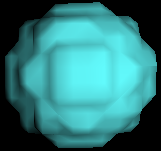
\includegraphics[scale=1.05]{figures/VoxelSphere/Radius5-0.png}
	}
	\subfloat[]{
		\hspace{0.5cm}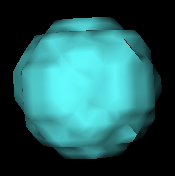
\includegraphics[scale=0.9]{figures/VoxelSphere/Radius5-1.png}
	}
	\end{center}
	\begin{center}
	\subfloat[]{
		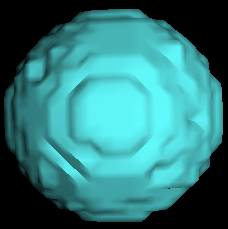
\includegraphics[scale=0.73]{figures/VoxelSphere/Radius9-0.png}
	}
	\subfloat[]{
		\hspace{0.5cm}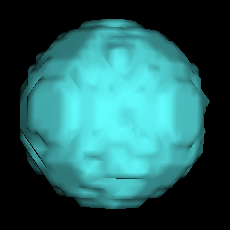
\includegraphics[scale=0.69]{figures/VoxelSphere/Radius9-1.png}
	}
	\end{center}
	\caption{\label{img:DrawnSphereCellRadius5And9}A single cell drawn into the simulation field. The radius of the cell of (a) and (b) is 5 and the radius of the cell of (c) and (d) is 9. Pictures (a) and (c) are with the front view, whereas the
pictures (b) and (d) have an view angle of around 45 degree. The color of the cell is chosen in
a way that more details are visible.}
\end{figure}

\begin{figure}
	\begin{center}
	\subfloat[]{
		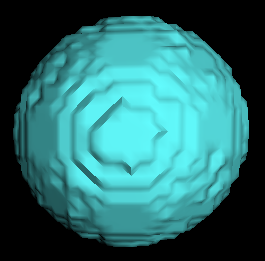
\includegraphics[scale=0.65]{figures/VoxelSphere/Radius14-0.png}
	}
	\subfloat[]{
		\hspace{0.5cm}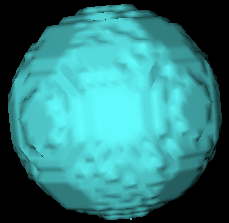
\includegraphics[scale=0.76]{figures/VoxelSphere/Radius14-1.png}
	}
	\end{center}
	\begin{center}
	\subfloat[]{
		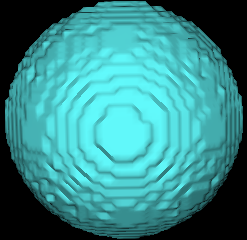
\includegraphics[scale=0.705]{figures/VoxelSphere/Radius23-0.png}
	}
	\subfloat[]{
		\hspace{0.5cm}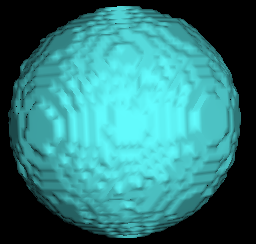
\includegraphics[scale=0.695]{figures/VoxelSphere/Radius23-1.png}
	}
	\end{center}
	\caption{\label{img:DrawnSphereCellRadius14And23}A single cell drawn into the simulation field. The radius of the cell of (a) and (b) is 14 and the radius of the cell of (c) and (d) is 23. Pictures (a) and (c) are with the front view, whereas the
pictures (b) and (d) have an view angle of around 45 degree. The color of the cell is chosen in
a way that more details are visible.}
\end{figure}


\newpage
\section{Calulate the voxel volume and surface sites of a sphere cell}
The created algorithm of section \ref{sec:CreatedAlgorithm} is able to calculate of a given radius the volume, of a sphere cell created with cuboids, in voxel as well as it is able to count the surface sites of the cell. Moreover, it is also possible to calculate the physical volume and surface of a sphere with a given radius. With this algorithm it is possible to calculate the volume and surface of a cell, drawn as a sphere of voxels, and become the same result as \ac{CC3D} calculates. \newline
The algorithm is useful but also has its weaknesses. For a voxel density beside 1 the results between the created algorithm and \ac{CC3D} deviate. The results differ also if the radius is not a whole number. There are no insights how \ac{CC3D} calculates the volume and surface of a drawn sphere cell. Moreover, for the tenths part of 5 to 9, for every radius with $.5$ until $.9$ it is possible to create the cube with an radius which is either rounded up or down. This means for a radius of $3.7$ it is possible to use either 6 or 8 voxels to create the cuboid, as the diameter is best as $2 \cdot r$. \newline
The algorithm helps to calculate the volume of a sphere cell, out of voxels, as well as to count the surface sites. It is able to be executed without an start of an simulaion. Thus, there is no need to adjust the coding of the project and to wait until the simulation started to recieve the volume and surface values of a cell drawn as a sphere out of voxels. 

\section{Grow sphere cells}
In section \ref{sec:GrowSphereCell} the factor for the calculation of the surface of the cell was evidenced best to be $1.5$. With this factor it should be possible to let the sphere cell grow as a sphere. To test the growth of the cell, one single cell was placed in the simulation field. As the cell growed during the simulation the volume and surface values were rad out of the command line and compared to the documented values of a drawn cell. \newline
To let a cell grow as a sphere does not work. Even the volume and surface values, calculated by \ac{CC3D}, and the target volume and target surface values, calculated by the program, meet the values of drawn sphere cells with a small deviation \textit{of an maximum deviation up to 50}.

Figures \ref{img:GrowthSphereCellRadius5} and \ref{img:GrowthSphereCellRadius9} display two examples of a single cell placed in the simulation field. It is observable that drawn sphere cells with a smaller radius become a cubish shape faster. In fiugre \ref{img:GrowthSphereCellRadius5} the cell has a cubish form after 50 \ac{MCS} where the cell in figure \ref{img:GrowthSphereCellRadius9} becomes cubish after 750 \ac{MCS}. This might be a result that the larger sphere cell has more detail than the cell with a smaller radius.

\begin{figure}
	\begin{center}
	\subfloat[]{
		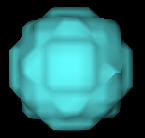
\includegraphics[scale=1.15]{figures/GrowthSphereCell/Radius5/Radius5-MCS0.png}
	}
	\subfloat[]{
		\hspace{0.5cm}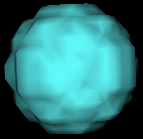
\includegraphics[scale=1.15]{figures/GrowthSphereCell/Radius5/Radius5-MCS0-1.png}
	}
	\end{center}
	\begin{center}
	\subfloat[]{
		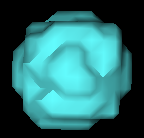
\includegraphics[scale=1.16]{figures/GrowthSphereCell/Radius5/Radius5-MCS50.png}
	}
	\subfloat[]{
		\hspace{0.5cm}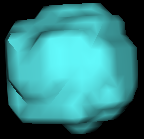
\includegraphics[scale=1.155]{figures/GrowthSphereCell/Radius5/Radius5-MCS50-1.png}
	}
	\end{center}
	\begin{center}
	\subfloat[]{
		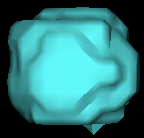
\includegraphics[scale=1.145]{figures/GrowthSphereCell/Radius5/Radius5-MCS250.png}
	}
	\subfloat[]{
		\hspace{0.53cm}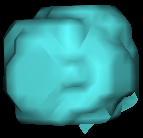
\includegraphics[scale=1.105]{figures/GrowthSphereCell/Radius5/Radius5-MCS250-1.png}
	}
	\end{center}
	\caption{\label{img:GrowthSphereCellRadius5}A sphere cell, with a radius of \SI{5}{\micro\metre} and a voxel density of 1, as it grows. Images (a), (c) and (e) are the front view of the cell and figures (b), (d) and(f) have around a 45 degree angle of the front. Figure (a) and (b) are at \ac{MCS} 0, images (c) and (d) at calculation step 50 and figures (e) and (f) present \ac{MCS} 250.}
\end{figure}

\begin{figure}
	\begin{center}
	\subfloat[]{
		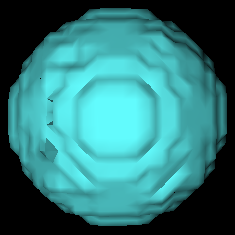
\includegraphics[scale=0.7]{figures/GrowthSphereCell/Radius9/Radius9-MCS0.png}
	}
	\subfloat[]{
		\hspace{0.5cm}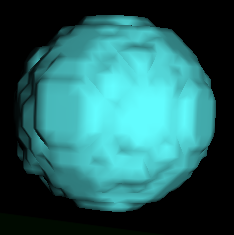
\includegraphics[scale=0.7]{figures/GrowthSphereCell/Radius9/Radius9-MCS0-1.png}
	}
	\end{center}
	\begin{center}
	\subfloat[]{
		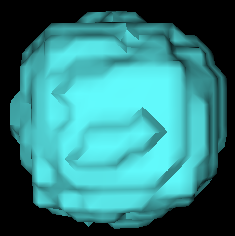
\includegraphics[scale=0.7]{figures/GrowthSphereCell/Radius9/Radius9-MCS750.png}
	}
	\subfloat[]{
		\hspace{0.5cm}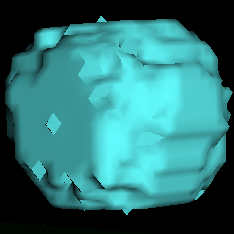
\includegraphics[scale=0.64]{figures/GrowthSphereCell/Radius9/Radius9-MCS750-1.png}
	}
	\end{center}
	\begin{center}
	\subfloat[]{
		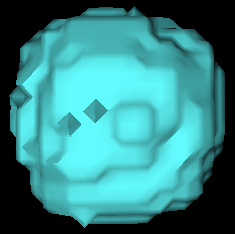
\includegraphics[scale=0.7]{figures/GrowthSphereCell/Radius9/Radius9-MCS1250.png}
	}
	\subfloat[]{
		\hspace{0.5cm}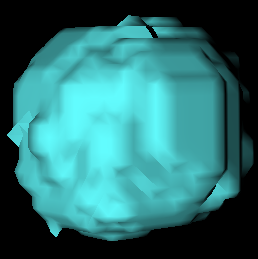
\includegraphics[scale=0.64]{figures/GrowthSphereCell/Radius9/Radius9-MCS1250-1.png}
	}
	\end{center}
	\caption{\label{img:GrowthSphereCellRadius9}A sphere cell, with a radius of \SI{9}{\micro\metre} and a voxel density of 1, as it grows. Images (a), (c) and (e) are the front view of the cell and figures (b), (d) and(f) have around a 45 degree angle of the front. Figure (a) and (b) are at \ac{MCS} 0, images (c) and (d) at calculation step 750 and figures (e) and (f) present \ac{MCS} 1250.}
\end{figure}

\section{Simulations}
Since no simulations are completed with three dimensions, several 3D simulations are presented. The models, which are simulated, are the most realistic models which were evidenced in an earlier version of the project \cite{Torelli2017}. The specific models are...